\documentclass[11pt,final,reqno]{amsart}
\addtolength{\textheight}{0.4in}
\addtolength{\topmargin}{-0.15in}
\addtolength{\oddsidemargin}{-.45in}
\addtolength{\evensidemargin}{-.45in}
\addtolength{\textwidth}{1.0in}

\renewcommand{\baselinestretch}{1.09}

\usepackage{bm,url,xspace,fancyvrb}
\usepackage{amssymb,amsmath}
\usepackage[final,pdftex]{graphicx}

%\usepackage[pdftex]{hyperref}

\newcommand{\ddt}[1]{\ensuremath{\frac{\partial #1}{\partial t}}}
\newcommand{\ddx}[1]{\ensuremath{\frac{\partial #1}{\partial x}}}
\newcommand{\ddy}[1]{\ensuremath{\frac{\partial #1}{\partial y}}}
\newcommand{\pp}[2]{\ensuremath{\frac{\partial #1}{\partial #2}}}
\newcommand{\eps}{\epsilon}
\newcommand{\grad}{\nabla}
\newcommand{\RR}{\mathbb{R}}

\newcommand{\bbF}{\mathbf{F}}
\newcommand{\bU}{\mathbf{U}}
\newcommand{\bY}{\mathbf{Y}}

\newcommand{\bb}{\mathbf{b}}
\newcommand{\bw}{\mathbf{w}}


\begin{document}

\title[On the PETSc code \texttt{ssaflowline.c}]{On the PETSc code \texttt{ssaflowline.c}, and its \\ residual, Jacobian matrix, and Picard preconditioner \\ components}
\author{Ed Bueler}
\date{\today}
\maketitle

These notes document the numerical choices made in the code \texttt{ssaflowline.c}.  This code, and these choices, should be compared to those in the Matlab/Octave codes \texttt{flowline.m}, \texttt{ssaflowline.m}, and \texttt{testshelf.m} in directory \texttt{mfiles/}, which are described in detail in the lecture.

\subsection*{Discrete residual}   The equation we solve is the no-basal-friction ($C=0$) version of the flow-line SSA stated in the lectures:
\begin{equation}
  \left(2 B H |u_x|^{p-2} u_x\right)_x - \frac{1}{2} \rho g (1-r) \left(H^2\right)_x = 0.  \label{ssa}
\end{equation}
The solution of this equation $u(x)$ is the velocity in the ice shelf.  This PDE\footnote{Actually the differential equation is a two-point boundary value problem for an ODE.  In many ways it is ``too simple''; see the last subsection.  But we treat it as a PDE as we are considering methods that generalize easily to true PDEs.} applies on the interval $0<x<L$ where $x=0$ is the location of the grounding line and $x=L$ is the location of the calving front.  It has these boundary conditions:
\begin{equation}
u\big|_{x=0} = u_g, \qquad\qquad \left[2 B H |u_x|^{p-2} u_x - \frac{1}{2}\rho g (1-r) H^2\right]_{x=L} = 0,
\end{equation}
where the thickness is a fixed function $H=H(x)$.  Note that $n$, $p=1+1/n$, $A$, $B=A^{-1/n}$, $\rho$, $\rho_w$, $r=\rho/\rho_w$, $u_g$, and $L$ are all positive constants.  The second boundary condition can be rewritten in the form we actually use,
\begin{equation}
u_x\big|_{x=L} = \gamma \qquad \text{where} \qquad \gamma = \left(\frac{\rho g (1-r)}{4B} H(L)\right)^n. \tag{2b} \label{neumann}
\end{equation}

We have clearly stated the continuum problem.  In addition to choosing a discretization scheme, the first goal is to construct the \emph{residual}, the amount by which a candidate solution to the discrete problem does not solve the discrete equations.  That is, instead of immediately formulating a scheme for solving the discrete equations, we first address the simpler job of merely measuring how wrong is any candidate (guess) for the solution.

We will discretize the problem by finite differences, on an equally-spaced grid of $M$ points $x_0,x_1,\dots,x_{M-1}$.  Let $\Delta x = L / (M-1)$ and $x_i = i \Delta x$.  The unknowns $U_i$ in the discrete problem (below) approximate the corresponding exact values on the grid $u(x_i)$, and form a vector $\bU = (U_0,\dots,U_{M-1})$.  So we now write the discretized PDE \eqref{ssa} and its boundary conditions as $M$ nonlinear equations in $M$ real unknowns:
\begin{align}
  0 = f_0(\bU) &= U_0 - u_g \tag{3a} \label{reszero} \\
  0 = f_1(\bU) &= \eta(U_2-U_1) H_{3/2} (U_2 - U_1) - \eta(U_1 - u_g) H_{1/2} (U_1 - u_g) \tag{3b} \label{resone}\\
               &\qquad - (\Delta x) K (H_{3/2}^2 - H_{1/2}^2) \notag \\
  0 = f_i(\bU) &= \eta(U_{i+1}-U_i) H_{i+1/2} (U_{i+1} - U_i) - \eta(U_i - U_{i-1}) H_{i-1/2} (U_i - U_{i-1}) \tag{3c}  \label{resi}\\
               &\qquad - (\Delta x) K (H_{i+1/2}^2 - H_{i-1/2}^2), \qquad [i=2,3,\dots,M-2] \notag \\
  0 = f_{M-1}(\bU) &= \eta(U_{M-2} + 2\Delta x \gamma - U_{M-1}) H_{M-1/2} (U_{M-2} + 2\Delta x \gamma - U_{M-1})  \tag{3d} \label{resend} \\
               &\qquad - \eta(U_{M-1} - U_{M-2}) H_{M-3/2} (U_{M-1} - U_{M-2}) \notag\\
               &\qquad - (\Delta x) K (H_{M-1/2}^2 - H_{M-3/2}^2) \notag
\end{align}
where $K = \rho g (1-r)/(4 B)$ and \setcounter{equation}{3}
\begin{equation}
  \eta(Z) = \left(\left(\frac{Z}{\Delta x}\right)^2 + \eps^2\right)^{(p-2)/2} \label{visc}
\end{equation}
The functions $f_i$ are called the \emph{residuals}.  They form a residual vector denoted $\bbF(\bU)$.

Some comments about equations (3) and \eqref{visc} are appropriate:\begin{itemize}
\item All equations, except the $i=0$ case \eqref{reszero}, are scaled by ``clearing denominators'', that is, by multiplying the discretized equation by $\Delta x^2$.
\item The $i=1$ case in equation \eqref{resone} is not quite in the general form \eqref{resi} because, for greater symmetry of the Jacobian matrix (below), the known value $u(x_0)=u_g$ at the left neighbor is used directly.
\item The $i=M-1$ case \eqref{resend} comes from introducing a ``virtual'' unknown $U_{M}$ and then approximating the derivative of the solution at the calving front by a centered difference formula:
  $$u_x(L) = u_x(x_{M-1}) \approx \frac{U_M - U_{M-2}}{2\Delta x}.$$
Both the calving front boundary condition \eqref{neumann} and the PDE itself \eqref{ssa} are enforced at $x=x_{M-1}$, which allows elimination (by-hand) of the virtual $U_M$ \cite{MortonMayers}.
\item The function $\eta(Z)$ is a viscosity, up to a scalar factor.  This viscosity is regularized in equation \eqref{visc} by a positive constant $\eps>0$, with value equal to the strain rate of a $1$ m/a velocity change over the full length $L$ of the ice shelf (200 km), so $\eps \approx 1.6 \times 10^{-13}\,\text{s}^{-1}$.   No division by zero can, therefore, occur in evaluating the viscosity, which is always positive and finite.
\end{itemize}

\subsection*{Newton's method and the Jacobian matrix}   In equations (3) we have written the discrete problem in the abstract form
	$$\bbF(\bU) = 0.$$
Newton's method (\cite{Pressetal}, subsection 9.6) is a well-known iterative technique for solving such systems of equations.  It works if the residuals are differentiable functions and the initial iterate is sufficiently close to the desired solution.

The method is usually written in ``update'' form,\footnote{\textsl{Remark}.  This form of Newton's method may not be familiar from calculus, so let's clarify.  If we were solving a scalar problem $f(u)=0$ then we would first write the linearization $\ell(u)=f(u_n) + f'(u_n)(u-u_n)$ and then the Newton step as $\ell(u_{n+1}) = f(u_n) + f'(u_n) (u_{n+1}-u_n) = 0$.  Solving for $u_{n+1}$ gives the calculus form of the iteration.  The form $f'(u_n) (u_{n+1} - u_n) = -f(u_n)$ is the direct analog of \eqref{newtonstep}.  When the scalar derivative $f'(u_n)$ is replaced by a square matrix $J(\bU_n)$, which may not have an inverse at some step $\bU_n$, and when we need to choose a numerical method to solve the linear system in \eqref{newtonstep}, it is desireable to \emph{not} write the name of the (generally dense) inverse matrix $J(\bU_n)^{-1}$.} as follows.  First we solve a linear system for the Newton step $\bw$, and then we actually update the approximate solution $\bU_n \to \bU_{n+1}$:
\begin{gather}
J(\bU_n) \bw = - \bbF(\bU_n), \label{newtonstep} \\
\bU_{n+1} = \bU_n + \bw \notag
\end{gather}
For each candidate solution $\bU$, the \emph{Jacobian} $J(\bU)$ is a matrix with entries
\begin{equation} \label{jacobiandefn}
J(\bU)_{ij} = \frac{\partial f_i}{\partial U_j}.
\end{equation}

The Jacobian matrix \eqref{jacobiandefn} is tedious to write down in detail, but we do it anyway.  The matrix is tridiagonal, and we only give the nonzero entries, as follows:
\begin{align*}
J_{00} &= 1 \\
J_{11} &= - H_{3/2}\, \omega(U_2-U_1) - H_{1/2}\, \omega(U_1-u_g) \\
J_{12} &= H_{3/2}\, \omega(U_2-U_1) \\
J_{i,i-1} &= H_{i-1/2}\, \omega(U_i-U_{i-1}) &&[i=2,3,\dots,M-2] \\
J_{i,i} &= - H_{i+1/2}\, \omega(U_{i+1}-U_i) - H_{i-1/2}\, \omega(U_i-U_{i-1}) &&[i=2,3,\dots,M-2] \\
J_{i,i+1} &= H_{i+1/2}\, \omega(U_{i+1}-U_i)  &&[i=2,3,\dots,M-2] \\
J_{M-1,M-2} &= H_{M-1/2}\, \omega(U_{M-2}+2\Delta x \gamma - U_{M-1}) + H_{M-3/2}\, \omega(U_{M-1}-U_{M-2}) \\
J_{M-1,M-1} &= - H_{M-1/2}\, \omega(U_{M-2}+2\Delta x \gamma - U_{M-1}) - H_{M-3/2}\, \omega(U_{M-1}-U_{M-2})
\end{align*}
where
	$$\omega(Z) = Z\, \eta'(Z) + \eta(Z)$$
is the derivative of the function $Z \mapsto Z\, \eta(Z)$ and
	$$\eta'(Z) = \frac{p-2}{\Delta x^2}\, Z\, \left(\left(\frac{Z}{\Delta x}\right)^2 + \eps^2\right)^{(p-4)/2}.$$

The nonzero pattern of the Jacobian matrix is symmetric (Figure \ref{fig:spyJ}), but the actual matrix is not because of the way the Neumann boundary condition is imposed.  Specifically,
    $$J_{M-1,M-2} = H_{M-1/2}\, \omega(U_{M-2}+2\Delta x \gamma - U_{M-1}) + H_{M-3/2}\, \omega(U_{M-1}-U_{M-2})$$
is not equal to
    $$J_{M-2,M-1} = H_{M-3/2}\, \omega(U_{M-1}-U_{M-2}).$$
For $i=2,3,\dots,M-3$ we do have $J_{i,i-1} = J_{i-1,i}$, however.  It is an advantage of the finite element method (FEM), relative to our finite difference methods here, that the Jacobian is symmetric if the FEM is applied properly.

\begin{figure}[ht] 
\begin{center}
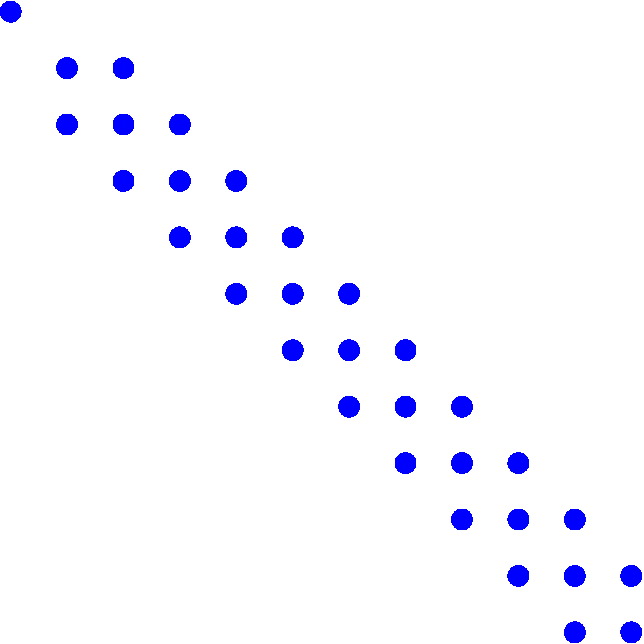
\includegraphics[width=0.25\textwidth]{spyJ}
\end{center}
\caption{Symmetric sparsity pattern of Jacobian matrix $J(\bU)$ for $M=12$.  The matrix itself is not symmetric, with $J_{M-2,M-1} \ne J_{M-1,M-2}$, as a consequence of the chosen finite difference implementation of the Neumann boundary condition at the calving front.}
\label{fig:spyJ}
\end{figure}

Newton's method comes with few guarantees.  It is generally not globally convergent.  This means that for some starting points the method may not converge to anything, or it may converge to a point which is not a solution of the equations.  There are, however, robust ``globalization'' techniques which greatly improve this aspect and make Newton's method very practical (e.g.~\cite{Pressetal}, subsection 9.7 sketches the Dennis \& Schnabel choice which we apply for equations (3)), and these techniques are available in PETSc (below).  

The very important advantage of Newton's method is that it is quadratically convergent---\emph{very fast} convergent---when the residual functions are twice-differentiable \cite{BurdenFaires}.  Properly-globalized Newton's method is known to work very fast on many nonlinear PDE problems, as long as good information is available to inform a choice of initial guess, and as long as attention is paid to the way the Jacobian is extracted and to the way the linear problem for the Newton step is solved.  That is our goal here.

\subsection*{Picard iteration, and its relationship to the Jacobian matrix} By considering the Newton method and the Jacobian matrix above, we have an apparently quite different way of solving our finite difference equations, compared to the Picard iteration used in the Matlab/Octave codes.  We show first that the difference is not as large as one might think, and then we show how to exploit the simpler matrix which appears in the Picard formulation, as part of the Newton step.

For the Picard iteration in the Matlab/Octave codes we could have written
\begin{equation}
	A(\bU_n) \bU_{n+1} = \bb \label{picardstepraw}
\end{equation}
from the discrete SSA equations in the form $A(\bU) \bU = \bb$.  In this case
	$$\bbF(\bU) = A(\bU) \bU - \bb$$
is the residual vector which we seek to make zero.

The Picard iteration can easily be written in the same form as the Newton step.  First we subtract $A(\bU_n) \bU_n$ from each side of \eqref{picardstepraw}:
	$$A(\bU_n) \bU_{n+1} - A(\bU_n) \bU_n = \bb - A(\bU_n) \bU_n.$$
Now we recognize $-\bbF(\bU_n)$ on the right side, factor the left side, and write the whole thing in update form:
\begin{gather}
A(\bU_n) \bw = - \bbF(\bU_n), \label{picardstep} \\
\bU_{n+1} = \bU_n + \bw \notag
\end{gather}
Form \eqref{picardstep} simply replaces $J(\bU_n) \to A(\bU_n)$ in \eqref{newtonstep}.

It is easy to extract the Picard matrix $A(\bU)$ from the residual-evaluation function which computes $\bbF(\bU)$.  We identify the coefficients, supposing that the viscosity is fixed at its values from $\bU$ at a previous step.  Again the matrix is tridiagonal:
\begin{align*}
A_{00} &= 1 \\
A_{11} &= - H_{3/2}\, \eta(U_2-U_1) - H_{1/2}\, \eta(U_1-u_g) \\
A_{12} &= H_{3/2}\, \eta(U_2-U_1) \\
A_{i,i-1} &= H_{i-1/2}\, \eta(U_i-U_{i-1}) &&[i=2,3,\dots,M-2] \\
A_{i,i} &= - H_{i+1/2}\, \eta(U_{i+1}-U_i) - H_{i-1/2}\, \eta(U_i-U_{i-1}) &&[i=2,3,\dots,M-2] \\
A_{i,i+1} &= H_{i+1/2}\, \eta(U_{i+1}-U_i)  &&[i=2,3,\dots,M-2] \\
A_{M-1,M-2} &= H_{M-1/2}\, \eta(U_{M-2}+2\Delta x \gamma - U_{M-1}) + H_{M-3/2}\, \eta(U_{M-1}-U_{M-2}) \\
A_{M-1,M-1} &= - H_{M-1/2}\, \eta(U_{M-2}+2\Delta x \gamma - U_{M-1}) - H_{M-3/2}\, \eta(U_{M-1}-U_{M-2})
\end{align*}

The careful reader will notice that the Picard matrix $A(\bU)$ is ``the same'' as the Jacobian matrix $J(\bU)$, with the replacement $\omega \to \eta$.  This is true, and indeed the only real simplification gained by considering the Picard matrix, compared to the Jacobian, is that the \emph{derivative} of the visosity $\eta(Z)$ is not needed.  This simplicity advantage of the Picard matrix becomes more significant with two or three spatial dimensions, as in more realistic ice shelf modeling.

\subsection*{Implementation in PETSc}  As pointed out in the lecture, the goal here is to demonstrate the use of the PETSc library \cite{petsc-user-ref}.  PETSc contains a rich set of linear and nonlinear solver tools which, unlike Matlab/Octave, ``scale up'' to handle the largest computations done in science and engineering.  On our problem, and problems like it, we are able to do build practical parallel simulations by writing code which works on sub-domains of our problem.  This subdomain code is then ``handed'' to the PETSc Newton solver object.  For PDE problems, PETSc codes for linear and nonlinear PDEs always demonstrate a parallel ``domain decomposition'' of the most basic sort.  Codes for nonlinear PDES always a residual evaluation routine.  One may also write routines which evaluate and assemble the Jacobian matrix or approximations to it (i.e.~Picard matrix in our case).

The C code \texttt{ssaflowline.c} contains these routines.  To build and run \texttt{ssaflowline.c} see Figure \ref{fig:buildrun}.  The code is intended for inspection by the reader.  It is hoped that this PETSc application is simultaneously simple enough and nontrivial enough so that the mathematical details do not hide the structure of the scientific computational tools.

\begin{figure}[ht]
\small
\begin{Verbatim}[xleftmargin=1in, frame=single]
$ cd karthaus/petsc/
$ source set_my_petsc
$ make
$ ./ssaflowline               # run it
$ ./ssaflowline -help |less   # see options
\end{Verbatim}
\normalsize
\caption{Build and run \texttt{ssaflowline.c}.  You will need to edit the file \texttt{set\_my\_petsc} to set your \texttt{PETSC\_DIR} and \texttt{PETSC\_ARCH} to the correct values for your PETSc.}
\label{fig:buildrun}
\end{figure}

The major components of the code \texttt{ssaflowline.c} are:
\begin{itemize}
\item \texttt{AppCtx}:\quad This structure is passed into the residual and Jacobian calculation routines so that these routines ``know about'' the constants set by default and by the user's options.  Also, for example, the gridded thickness values are here so that they can be used in the calculations.
\item \texttt{FillThicknessAndExactSoln()}:\quad As described in the lectures, we are solving for velocity in a steady-state case where both the exact ice thickness and velocity can be computed by-hand.  This routine computes both of these fields.  The exact velocity is only used for evaluating the numerical error.
\item \texttt{FormInitialGuess()}:\quad As described in the lectures, we can use a linear function as a guess for the velocity.  This initializes the Newton iteration.  (Option \texttt{-ssa\_guess 2} allows use of the exact solution as an initial guess.  This is useful for debugging.)
\item \texttt{FormFunctionLocal()}:\quad  Routine which calculates the residual $\bbF(\bU)$ from the current value of the solution  (in the Newton iteration).  The goal of the Newton method object (\texttt{SNES snes} in \texttt{main()}) is to make this residual zero.
\item \texttt{FormTrueJacobianMatrixLocal()}:\quad Calculates the Jacobian matrix $J(\bU)$ from the current value of the solution.
\item \texttt{FormPicardMatrixLocal()}:\quad Calculates the Picard matrix $A(\bU)$ from the current value of the solution.
\item \texttt{main()}:\quad  Reads options and sets up \texttt{AppCtx user}.  Based on options, sets up \texttt{SNES snes}, \texttt{DA user.da}, and related \texttt{Vec}s.  Calls \texttt{SNES} routines to set the method for computing the Jacobian, based on user options.  Ask the SNES object to solve the equations, by Newton's method, and gets/displays feedback on iterations and convergence.
\end{itemize}

The ``\texttt{Local}'' which appears in the names of the calculation routines (above) relates to the PETSc \texttt{DA}=(distributed array object) which does the domain decomposition across the grid.  The solution, the residual, and the thickness functions are all PETSc \texttt{Vec} objects, which are (conceptually) vectors in $\RR^M$, but which are distributed across processors according to the information in the \texttt{DA}.

For additional understanding of \texttt{ssaflowline.c}, the user should see the source code itself and read the \emph{PETSc User's Manual} \cite{petsc-user-ref}, especially the descriptions of \texttt{Vec}, \texttt{Mat}, \texttt{DA}, and \texttt{SNES} objects.

``Under the hood'' of the example done here is a PETSc \texttt{KSP} object which runs a Krylov subspace iterative linear solver.  We use the PETSc default \texttt{KSP} choice of GMRES because, in part, our Jacobian and approximate Jacobians are not symmetric.  The \texttt{KSP} is called when the \texttt{SNES} object managing the Newton method needs to solve a linear system for the step $\bw$.  Thus using \texttt{SNES} \emph{automatically} produces an outer/inner iteration structure.

To write a first-draft PETSc code on a problem like the one here, one writes a residual calculation routine plus minimal PETSc structure.  I have kept this first draft, namely \texttt{ssaflowline\_v0.c}.  There are nonlinear equation solution techniques which do not need the bug-prone assembly of Jacobian (or Picard, or any other) matrices.  In fact, with this most-minimal code we can try two methods:\renewcommand{\labelenumi}{\emph{\roman{enumi})}}
\begin{enumerate}
\item Option \texttt{-snes\_mf}:  A matrix-free form of the Newton method known as unpreconditioned ``Jacobian-free Newton-Krylov'' for domain decomposition problems \cite{KnollKeyes2004}.  It is a significant technique because, when appropriately used, it may be the the key to petaflops-level scientific simulations.  Actually making it scale requires building something matrix-like as a preconditioner, however, and we do that below.
\item Option \texttt{-snes\_fd}:  Naive finite differencing of the residual evaluation routine to construct an approximate Jacobian.  An un-necessarily large matrix is assembled, for a PDE problem like the one here.
\end{enumerate}

In using the first-draft with the above options it became clear that the residual evaluation gave an improved approximate Jacobian if the Dirichlet boundary condition at the grounding line was applied symmetrically, so that the $i=1$ residual equation looked like \eqref{resone} instead of the form it had in \texttt{ssaflowline\_v0.c}, namely
	$$0 = f_1(\bU) = \eta(U_2-U_1) H_{3/2} (U_2 - U_1) - \eta(U_1 - u_0) H_{1/2} (U_1 - U_0).$$

The first draft was improved to the final code \texttt{ssaflowline.c} in several other ways.  I added user options setting most parameters at runtime.  Then, because method \emph{ii)} above for computing the finite difference Jacobian can be improved greatly by giving PETSc the information that unknown $U_i$ depends only on unknowns $U_{i-1}$ and $U_{i+1}$, I supplied a \emph{coloring} for the finite-difference method; see \cite{petsc-user-ref}.  (The \texttt{DA} object knows the details and I did not write anything subtle, but there is a bit of set up.)

Then I added a Picard evaluation routine.  Even though this is not the true Jacobian, it can be used with option \texttt{-snes\_mf\_operator} to get much of the effect of the true Jacobian; see below.  Finally, I added a true Jacobian evaluation routine.  The default for \texttt{ssaflowline} is to use this true Jacobian.

With these additions there are three more computational paradigms to try; we continue the enumerated list above.  Note that options with prefix ``\texttt{ssa\_}'' are new in \texttt{ssaflowline.c}, and are not in PETSc itself:
\begin{enumerate}
\setcounter{enumi}{2}
\item No option:  Use the true, assembled Jacobian.  It can be used with various built-in preconditioning methods controlled by option \texttt{-pc\_type}.  The default preconditioner on one process is ILU.  The default for parallel runs is block Jacobi with ILU on the blocks.
\item Option \texttt{-ssa\_fd}:  Use a \texttt{DA}-based coloring routine to compute the finite difference approximation to the Jacobian much more efficiently.
\item Option combination \texttt{-snes\_mf\_operator -ssa\_picard}:  Assemble the Picard matrix, but then use it only as a preconditioning matrix in applying the Krylov method, while still computing the effect of the Jacobian by the matrix-free method.  For large-scale ice flow problems we should believe that this is a key technique, because the Jacobian evaluation means complex, bug-prone code, which may not even be possible to write when many physical processes are interacting, yet a rough, approximate Jacobian used as a preconditioner suffices to accelerate the matrix-free application of the Jacobian to a vector \cite{KnollKeyes2004}.
\end{enumerate}

\subsubsection*{Irritating detail}  On one of my first attempts using the unpreconditioned matrix-free method yielded a divergence error, despite coming close to the exact solution by reported errors.  This is resolved with an obscure option which modifies the way the matrix-free Jacobian is applied (to use a different step-size algorithm):
\begin{Verbatim}[fontsize=\small]
$ ./ssaflowline -snes_mf
...   DIVERGED_LS_FAILURE Number of Newton iterations = 6
  numerical errors in velocity: ...   2.5481e-02 relative maximum
$ ./ssaflowline -snes_mf -mat_mffd_type ds
...   CONVERGED_FNORM_RELATIVE Number of Newton iterations = 4
  numerical errors in velocity: ...   1.3373e-02 relative maximum
\end{Verbatim}


\subsection*{Results}  We want to know that our method, which is to say our actual code, is correct.  There are two important aspects to this.  We claim we are solving equation \eqref{ssa}, so one aspect is \emph{verification}, to measure difference between the final numerical result of our code and an exact solution, in a case where the latter is available.  The other aspect is the quadratic convergence mentioned above: if we have constructed a good initial quess and we have chosen a reasonable preconditioning routine then we will see that the Newton steps cause rapid convergence even for large problems.

So I did runs that looked like this:
\begin{Verbatim}
./ssaflowline -snes_monitor -snes_rtol 1e-12 -ksp_rtol 1e-12 -da_grid_x M
\end{Verbatim}
for values $M=10,100,10^3,10^4,10^5$ and in all runs the \texttt{SNES} object reported convergence.  These are single process runs; parallelization is not yet the issue.  The $M=10^5$ run only takes 1.2 seconds on my laptop, so raw performance on this 1D problem is also not an issue!

The verification results from these runs in Figure \ref{fig:numerr} show that once we reach $M=10^4$ we are getting results correct to about 6 digits, relative to the exact solution.  The 2 m grid with $M=10^5$ gives no more accuracy in this sense than the 20 m grid with $M=10^4$.

Figure \ref{fig:quadconv} gives the evidence for quadratic---more properly superlinear---convergence of the ``outer'' nonlinear iteration managed by the \texttt{SNES} object.  That is, Newton is working.  Note that if the residual norm was decaying exponentially in iteration number (= ``linear convergence'' \cite{BurdenFaires}), $\|\bbF(\bU_n)\| \sim \alpha^n$ for $\alpha < 1$, then Figure \ref{fig:quadconv} would show straight lines for each $M$.  But in all cases the residual norm decays at an increasing rate, until we reach the level controlled by linear iteration tolerance, rounding error, and condition number of the discrete nonlinear problem.  Thus we have probably written the correct Jacobian!

\begin{figure}[ht] 
\begin{center}
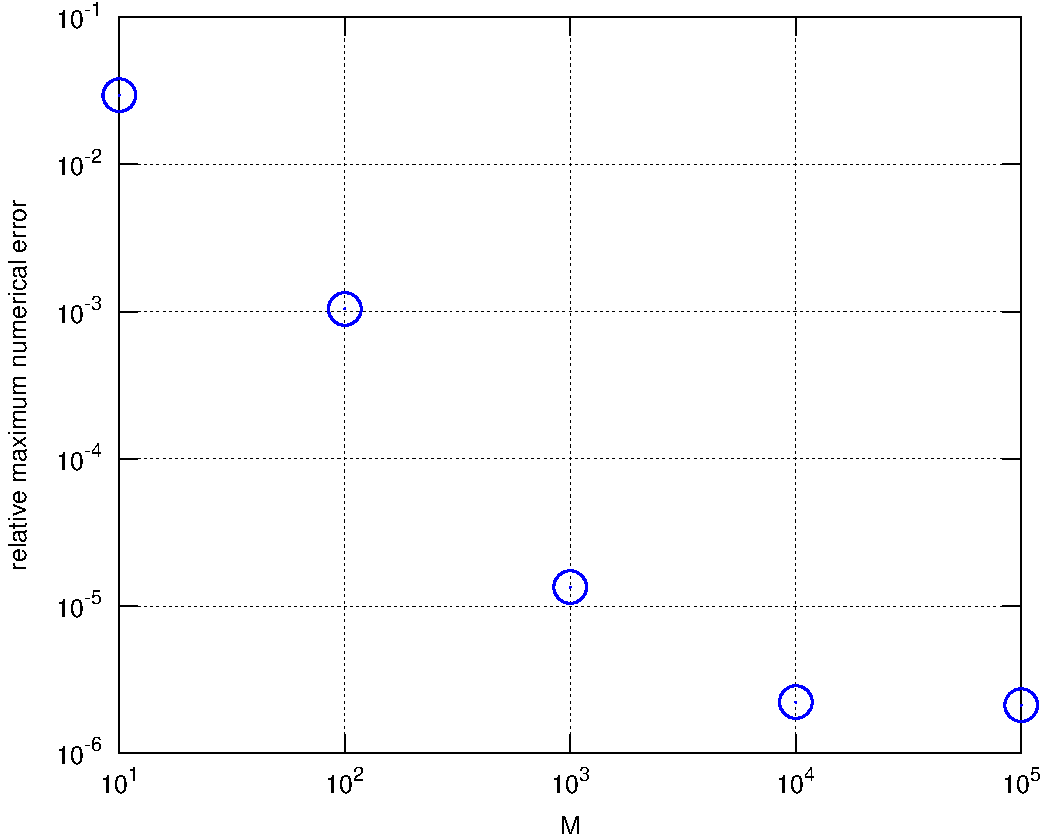
\includegraphics[width=0.5\textwidth]{numerr}
\end{center}
\caption{Verification:  Grid refinement ($M=10,100,10^3,10^4,10^5$) produces reduction in numerical error, relative to exact solution, and measured by comparing the maximum velocity error anywhere on the grid to the largest velocity.}
\label{fig:numerr}
\end{figure}

\begin{figure}[ht] 
\begin{center}
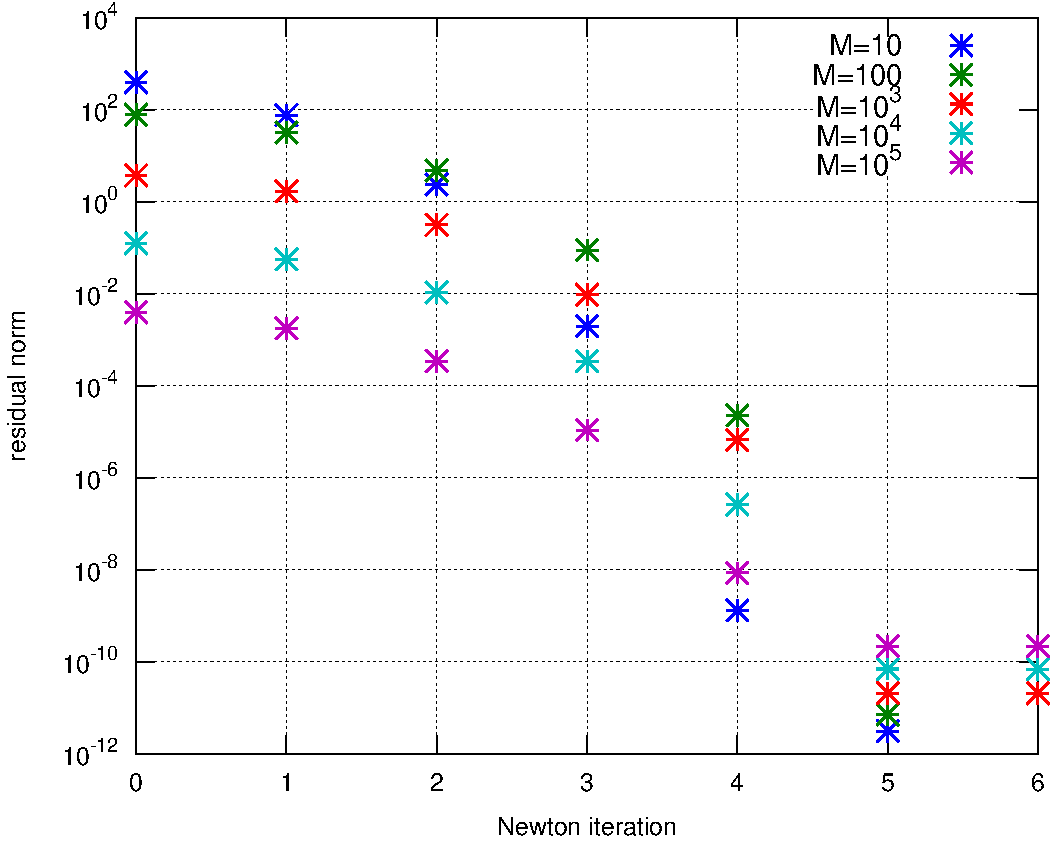
\includegraphics[width=0.5\textwidth]{quadconv}
\end{center}
\caption{Evidence of quadratic, or at least super-linear, convergence:  The residual norm decays faster than linearly with iteration number (i.e.~faster than $(\text{residual norm})\sim \alpha^n$ where $n$ is the iteration count).  Note that on the coarsest grid ($M=10$) we see the most rapid convergence to level $10^{-14}$ smaller than the initial residual norm.}
\label{fig:quadconv}
\end{figure}

Our code runs just fine on many processors.  For example,
\begin{Verbatim}
    $ mpiexec -n 10 ./ssaflowline -da_grid_x 10000
\end{Verbatim}
on ten processes computes the a solution with the same accuracy as on one ($2.2284\times 10^{-6}$ versus $2.2284\times 10^{-6}$ relative maximum error).  But are we getting a benefit from this parallelism?

For a large-scale problem there are several measures of parallel computational performance which we could now be interested in.  One might measure the number of linear iterations, the number of floating-point operations, or the actual (``wall clock'') time needed to solve a large problem in parallel.  For real problems we want to see performance which will scale up to apply to models covering large parts of realistic ice sheets at high spatial resolution.  This surely reflects the main goal of using a toolkit like PETSc for ice sheet modeling.  An example for ice sheet modeling is in \cite{BBssasliding}; see figure 24.

The time has come to admit, however, that the 1D ice shelf problem addressed here in these notes is \emph{too simple}.  Actually measuring computational performance in this example does not illustrate what happens to 2D and 3D problems, for these reasons:\begin{enumerate}
\item The matrices here are tridiagonal, which means that a default preconditioner (ILU) is both exact \emph{and} fast on one process.  The default block-Jacobi-plus-ILU-on-blocks choice in parallel is inexact, and thus much less fast because actual iterations must occur, on more than one process.  Having more than one process is therefore disadvantageous on this simple problem because the preconditioned-KSP no longer solves in just one iteration.  (In other words, PETSc is ``wise'' and reverts to the obvious best choice for a diagonally-dominant tridiagonal problem!)
\item The domain is one dimensional but the modeled physical process, namely the resolution of stresses in an ice shelf, is long range.  Dividing a roughly-square, 2D ice shelf region among 100 processes requires effects to be communicated across (through) 10 processes.  But here in 1D the effect must ``domino'' through all 100 processes if we choose to use that many.
\end{enumerate}

Finally we point out a basic, positive benefit of our efforts here: compiled C code runs a lot faster than interpreted Octave, as expected.  This run
\begin{Verbatim}
    $ ./ssaflowline -da_grid_x 200000
\end{Verbatim}
on a 1 m grid ($M=2\times 10^5$ points with length $L=200$ km) returned a numerical velocity field that was correct to a relative error of $2\times 10^6$.  It completed in 6 Newton iterations and about 2 wall clock seconds.  By contrast, the $M=4000$ case for the Octave code \texttt{testshelf.m} took 16 seconds and returned an answer correct to $5 \times 10^6$.  The fact that our code uses PETSc is probably not very important in this regard.

\subsection*{Acknowledgements}  Help from Jed Brown was central to building this example.

\bibliography{ice_bib}
\bibliographystyle{siam}

\end{document}
